%------------------------------------------------------------------------
\chapter{3D Model of Object Context}
\label{3DModelofObjectContext.ch}
%------------------------------------------------------------------------
%revised 21-02-13
\section{An example Scenario}
\label{Scenario.sec}
% Point-clouds get captured
% Apply the models on the point-clouds
% By matches for models that are found, we know what object classes should be expected in that place
% Based on this result and the ground truth for each place category, the probability of belonging the place to each category is estimated.

In this scenario, a situation is considered where a mobile robot wants to look around in a building and make a map including semantic information about the 
places that it meets in the map. 
The robot builds a 3D map of the building using, for instance, a SLAM application. 
Employing the context models, which has been trained for different key object classes, the robot can estimate which object classes 
are probable to be found in each place that is present in the map. 

By key objects we are referring to distinctive objects for a place category. These specific object classes should be chosen based on 
a ground truth which is defined in advance for a place category. It is discussed in Chapter ~\ref{UsingObjectContextforPlaceClassification.ch}
in more detail.

Then using the results, showing which object classes are expected in a place and based on the ground truth, for key objects of each place
category, the place is classified. 

% But for the building of the model it self. the same steps mentioned above for capturing the point cloud would be performed,
% on the pre processed captured point cloud of a place using the annotation tool we have developed, key objects for that 
% specific place category would be annotated. Feature extraction would be run on this annotated point cloud giving training 
% samples. Train samples would be combined from several different point-clouds for the same place category but different 
% instances, Resulting data set would be divided into train, validation and test sets. Using SVM with two kernels the model would be 
% trained.
% 
% More details would be presented in section ~\ref{Implementation.sec}

\section{Implementation}
\label{Implementation.sec}

In this Section, the procedure of building the context model and how it is applied, is described in detail. 
The input in this procedure is the point-cloud of a scene and the output is a list of probability values assigned to all regions in
the scene. 
The probability value shows if the region is likely to be a context. 
The input cloud is first preprocessed and then get annotated with instances of the object class whose context model is being built. 
Feature extraction would be run on this annotated point-cloud and result in the train samples. 
Train samples would be combined from several different point-clouds for the same object class to make the Train Set. 
Then the Train Set is given to SVM classifier to make the Context Model. A block diagram in figure ~\ref{SystemOverview.figure} shows 
the system overview.

\begin{figure}[t]
  \centerpsw{SystemOverview}{0.8\columnwidth}
  \caption[System Overview]
  {The overview of the system. Box on the left side shows the Train part of the system while the one on the right shows the prediction part.}
  \label{SystemOverview.figure}
\end{figure}

In the following Subsection First, we introduce the features used in this work and description of the modules of the system 
will come next.

% Features used
The data type we used in this work is PCL point-cloud ~\cite{Rusu_ICRA2011_PCL}. 
In this data type 3D coordinates and color information of a point is saved in a record and then an array of these records forms 
the point-cloud.
We used Microsoft Kinect with OpenNi driver to capture these point-clouds. 

%TODO: define terms used in the report, like blob

The feature vector we used consists of 2 parts. 
The first part includes two fields : First is the average height of the blob from which the features are extracted with respect to
the floor. 
The Second field is the orientation of the blob with respect to the vector of gravity. 
And the rest of the fields are in second part of the feature vector which is a histogram.
This histogram is called VFH which captures the geometry of the blob with respect to a specific view point. ~\cite{5651280}

\subsection{The Viewpoint Feature Histogram (VFH)}
\label{VFH.ssec}

As it is described in PCL official website ~\cite{VFH_Definition} and ~\cite{5651280}, 
VFH consists of two component as follows:

\begin{itemize}
 \item First component is a histogram for viewpoints(128 bins)
 \item Second component is extended Fast Point feature histogram(FPFH:4*45 bins)
\end{itemize}

The viewpoint component is computed as a histogram of the angles that direction of the viewpoint  makes with each surface
normals. 
It is important to notice that, this angle is between the central direction of the viewpoint and the normal, not the view angle of
the normal which would have made it not scale invariant. 

\begin{figure}[t]
  \centerpsw{ViewPoint_component}{0.8\columnwidth}
  \caption[ViewPoint Component of VFH]
  {Viewpoint part of the feature vector.\cite{VFH_Definition}}
  \label{VFH_ViewPoint_component.figure}
\end{figure}

The second component measures the relative pan, tilt and yaw angles that are measured between direction of the viewpoint  at the 
central point and each of the normals on the surface. 
So it consists of accumulated FPFH values for points in the query point-cloud.
That is why it is referred here as extended FPFH.

FPFH or Fast Point Feature Histogram itself can be considered as a revised version of PFH. FPFH reduces the complexity 
of PFH algorithm from $ O(n k^{2}) $ to $ O(n k) $ where $n$ is the number of points in the query point-cloud and $k$ is 
the number of points in the considered neighborhood of each query point. 
%This is the reason why it is called Fast PFH.
Although it reduces the informativeness of the feature but it would be still enough powerful and impressively faster 
to compute. 

PFH captures 3D geometry of the surfaces around a query point and it is invariant to the 6D pose of the query blob's 
surface. 
It is robust to different sampling densities or noise levels in the neighborhood of the query point. 
The descriptor is computed by estimating a histogram with concatenated 45 bins for four different element measured for every 
possible pairs of points in the query point's neighborhood ($ O(n k^{2}) $). 
The elements consist of three angles and a distance. 

In FPFH \cite{FPFH_Definition}, instead of encoding this information for all pairs of points in a neighborhood, It will only 
take pairs between the query point and its neighbors ($ O(n k) $). 
At this stage it is referred to as simplified PFH or SPFH. 
Then to keep the amount of information that this feature can provide, it also estimates SPFH for all $k$ points in the neighborhood.
The resulting values are integrated with a normalization to result in the FPFH of the query point(equation ~\ref{FPFH.eq}).

\begin{equation}
 \label{FPFH.eq}
 FPFH(P_{q}) = SPFH(P_{q}) + \frac{1}{k} \sum_{i=1}^k {\frac{1}{\omega_k}} \cdot SPFH(k)
\end{equation}


Figure  ~\ref{FPFH.figure} shows the encoded elements and their relation in FPFH.

\begin{figure}[t]
  \centerpsw{fpfh_component}{0.65\columnwidth}
  \caption[FPFH elements.]
  {Three angles and a distance encoded in FPFH and the points considered.\cite{VFH_Definition}}
  \label{FPFH.figure}
\end{figure}

Finally, in VFH the resulting FPFH of points in the point cloud are integrated to produce one of the two components(extended FPFH).
The histogram in this component has 180 bins (4*45 bin).
By adding the view point component (128 bin), it produces a 308 bin histogram. 
Unlike FPFH, as a result of adding the viewpoint component VFH is dependent to viewpoint but it still preserve the property of 
being scale invariant. 
Figure ~\ref{VFH_plot.figure} shows a sample plot of VFH and its components.

\begin{figure}[t]
  \centerpsw{vfh_histogram}{0.65\columnwidth}
  \caption[VFH histogram]
  {A sample plot of VFH and its components.\cite{VFH_Definition}}
  \label{VFH_plot.figure}
\end{figure}

The images and definitions are taken from Point Cloud official website.

% Libraries
\subsection*{Used Libraries in Implementation}

Most of the implementation is done in C++. 
There are some scripts for evaluation part of the results and creating the dataset for experiments written in MATLAB and also 
scripts creating the experiments and the experimental environment are in python. 
Libraries used in this work are as follow:

\begin{itemize}
 \item PCL \cite{Rusu_ICRA2011_PCL}
 \item Eigen \cite{eigenweb}
 \item LIBSVM \cite{LIBSVM}
\end{itemize}


\subsection{System Modules}
As illustrated in figure ~\ref{SystemOverview.figure}, apart from SVM there are three modules in the system:

\begin{itemize}
  \item PreProcess
  \item Annotation
  \item FeatureExtract
\end{itemize}

\subsubsection{PreProcess}
\label{PreProcess.ssec}
 In this module, the input point-clouds get prepared for annotation and feature extract. 
 The point-clouds we used in this work are saved in "PCD" format and their point type is PointXYZRGB which is PCL point type. 
 The processes for capturing these point-clouds is discussed in Section ~\ref{ExperimentalSetup.sec}. 
 First step in preparation of the input is transforming it.
 Based on the location and orientation of the sensor in time $t_0$ the resulting point cloud is transformed from sensor coordinate 
 system to the world's coordinate system. 
 As a different PCL point type is used in the rest of the process, in this step a conversion of the transformed point-cloud into that type 
 is also carried out.
 
 This new point type is PointXYZRGBL which includes a field in each point for label which is used later in annotation 
 tool and also in feature extract to decide about the class of the sample in train data set. 
 The most important step, which is taken here is estimation of surface normals which is essential for feature extraction. 
 The accuracy of the VFH feature is directly dependent to the accuracy of the normals. 
 %At first we were doing this process in feature extract module and for each query blob at the moment which added a huge overhead to
 %the process while it could be done independently and once for each point cloud. 
 Here the normals for the whole point cloud is estimated once and saved in a separate pcd file to be used in feature extract. 
 %It uses NormalEstimation class in PCL.
 
 There is also one more product for this module, which is discussed more in ~\ref{FeatureExtract.ssec}.
 It is a generated point-cloud which preserves size of the input cloud while complementing points, with respect to the input cloud,
 are added in it. It is used as a source for picking viewpoints that are needed in feature extraction.
 
 Therefore, the results of this module are as follows:
 \begin{itemize}
  \item Point-cloud's normals
  \item The transformed version of the input cloud
  \item Converted version into PointXYZRGBL
  \item TFP-cloud
 \end{itemize}
 
\begin{algorithm}[t]
\begin{algorithmic}[1]
\REQUIRE Input Point-cloud(XYZRGB).
\REQUIRE Sensor Location and orientation.
\medskip

\STATE Transfer the input cloud based on Sensor location and orientation from camera coordinate to world coordinate, and store the 
result.
\STATE Estimate Normals and store.
\STATE Convert the Pointcloud\_Transfered to Point type XYZRGBL and store in Pointcloud\_Converted.
\STATE Estimate 3DMINMAX of the Pointcloud\_Converted.
\STATE Using result from previous step, generate TFP pointcloud.

\medskip
\ENSURE Pointcloud\_Transfered.
\ENSURE Pointcloud\_Normals.
\ENSURE Pointcloud\_Converted(XYZRGBL).
\ENSURE Pointcloud\_Generated(TFP).

\end{algorithmic}
\caption[PreProcess.]
{A brief algorithmic description of PreProcess.}
\label{Preprocess.algorithm}
\end{algorithm}



 
 
\subsubsection{Annotation}
\label{Annotation.ssec}
In this module the PointXYZRGBL version of the point-cloud is loaded to get annotated. 
The objects needed to be annotated in the scene, are selected by clicking roughly on their center. 
The labels of the points belonging to them are assigned with a value representing object points. 
Objects from different classes could be labeled with different values (\ref{Annotation.algorithm}).

\begin{algorithm}[t]
\begin{algorithmic}[1]
\REQUIRE Pointcloud\_Transfered(XYZRGB).
\REQUIRE Object radius(rough estimate).
\medskip

\STATE Visualize input cloud.
\FORALL{objects to be annotated}
  \STATE Run Point picking procedure.
  \STATE Extract neighbor points indexes with respect to the input object radius.
  \STATE Label points whose indexes are extracted in previous step.
\ENDFOR
\STATE Store the pointcloud with the labels in output cloud.

\medskip
\ENSURE Pointcloud\_Annotated(XYZRGBL).
\end{algorithmic}
\caption[Annotation.]
{A brief algorithmic description of Annotation.}
\label{Annotation.algorithm}
\end{algorithm}


Figure ~\ref{TrashbinBounding.figure}, shows a scene in an office at KTH. 
The object of interest here is the trash bin, which is marked by a green bounding box. 
This figure is an image of the scene whose point-cloud is available in our dataset and the annotation is done on the point-cloud. 
In figure ~\ref{Annotation.figure} the annotated object could be seen in red within the scene's point-cloud.
It can be seen that some part of the floor is also colored in red, which means that part of the floor is also annotated as the object.
The reason is the object radius, that is given to annotation tool was not accurate enough or the center of the object was not 
picked accurately.
But it does not harm the result and this much of accuracy is more than enough.
Usually annotation is done using a bounding box which consider the box surrounding the object as the object.
Here, we exactly separate the points of the object by benefiting from the 3D coordinates of the points in the point-cloud.

\begin{figure}[t]
  \centerpsw{TrashbinBounding}{0.65\columnwidth}
  \caption[Example scene and object for Annotation tool]
  {An example scene and a trash bin marked by a bounding box as the object which is being annotated (Best viewed in color).}
  \label{TrashbinBounding.figure}
\end{figure}

\begin{figure}[t]
  \centerpsw{Annotation}{0.65\columnwidth}
  \caption[Annotation tool result]
  {An example of annotation result on the point-cloud, red points assumed to belong to the object(Best viewed in color).}
  \label{Annotation.figure}
\end{figure}

This package is available with source to be used by other researchers and get improved by developers.\cite{AnnotationGithub}

% Feature extraction

\subsubsection{FeatureExtract}
\label{FeatureExtract.ssec}
First, we Introduce some terms used in this part. They are as follows:
\begin{itemize}
  \item Blob: A sub set of the Point-cloud which includes a number of points in a neighborhood within a specific radius.
  \item Query Blob: The blob from which the features are being extracted.
  \item QPoint: The Query Point that is the center of the query blob. It is a point on the context of the object.
  \item OPoint: The Object point is the point in surrounding of the Qpoint which is an object point in a positive sample.
 \end{itemize}
 
 Instances of these elements are illustrated in Figure ~\ref{FEStructure.figure} for the example scene that we saw in Figure 
 ~\ref{TrashbinBounding.figure}. 
 The red point in the figure shows the $Query$ $Point$, which is a point picked from the context of the object and the features are extracted from the sphere surrounding it. The sphere is also visible in the figure which is the 
$Query$ $blob$. 
 The yellow point is the $OPoint$ or object point which is a point on the annotated object. 
 
 \begin{figure}[t]
  \centerpsw{FEStructure}{0.65\columnwidth}
  \caption[Illustration of the items used in Feature Extract.]
  {Structure used in Feature extraction; The red point is the QPoint; The sphere surrounding it, is the Query Blob; The yellow
  point is the OPoint (Best viewed in color).}
  \label{FEStructure.figure}
\end{figure}
 
In this module, the converted and transformed point-cloud and its normals are loaded.
To build the data set for train or test, Features are extracted for a number of keypoints from all over 
the point-cloud. 
The goal here is to get samples which are useful in building the context model for objects of interest. 
This is done in a way that for each key point, which is considered as a QPoint when it is selected for feature extract, 
we take a neighborhood of points and their corresponding point-normals to extract features from (Query Blob). 
%So thing that happens here is studding the geometry around the query point as a candidate geometry of a positive context.

The important idea applied here is the view point used in VFH.
For each QPoint and its corresponding Query blob, a number of points in a radius from the QPoint is considered as the view points 
(OPoints).
A sample is extracted for each pair of $Qpoint$ and $Opint_i$.
This way due to the difference in viewpoint, the features extracted for a single query point and its query blob would be slightly 
different. 
This will result in discrimination between same context viewed from different view point which is to our benefit.

As mentioned above, these view points are candidates for being object points.
In each sample if the OPoint in a pair of $(QPoint,OPint)$, is actually an object point we want this sample to be labeled as 
a positive sample and if not, to be a negative one. 
%This means that if the features are extracted from a query blob and for a view point which is within a specific distance from it,
%is located on the object of interest the query blob is actually a context for that object.
The view point also can help to encode the most probable location of the object with respect to the positive context. 

Another important point here is that we want the model to be able to locate candidates for context in a test point-cloud where 
object may be not present at the moment but its context is.
Therefor, we need the OPoints to be independent from actual points in the point-cloud.

This is where TFP-cloud finds it role.
This is a point-cloud generated in accordance to the input point-cloud which includes points with fixed structure to be used as 
candidate OPoints in feature extract.
Using these points as OPoints, we have fixed view points to sample the context for. 
To have the same structure in train and test data, we use the same OPoints in feature extract for train set as well.
The only difference in feature extract for train and test is that in train it is checked if the OPoint is on the object, using 
labels from annotated cloud. 
Then, if the answer is positive, the extracted sample would be a positive one. 
If not, it would be a negative sample. 
But in feature extract for test, we just do not do this check.

QPoints would be selected in a loop on key points in the point-cloud. 
The key point selection is done using VoxelGrid with a radius that would be dependent to the size of the object of interest. 
This way, we have a normally distributed key points in the input point-cloud which will make the sampling more informative.

For each of these QPoints, a blob around them is considered from the input cloud with point normals(Query blob).
In another loop, the OPoints are assigned  as the view point in feature extraction of each sample. 
Feature vector would be extracted for this blob and the OPoint. 
Figure ~\ref{PointParameters_Diagram.figure} shows these points and their related parameters. 
The values mentioned in the figure is for an example object class.

\begin{figure}[t]
  \centerpsw{PointParameters_Diagram}{0.65\columnwidth}
  \caption[Feature extract structure]
  {QPoint and generated OPoints and their spacial relations.}
  \label{PointParameters_Diagram.figure}
\end{figure}

\begin{algorithm}[t]
\begin{algorithmic}[1]
\REQUIRE Pointcloud\_annotated or Pointcloud\_converted(Depending train or test).
\REQUIRE Pointcloud\_Normals.
\REQUIRE Pointcloud\_Generated.
\REQUIRE S\_Radius
\REQUIRE OPoint\_Radius
\medskip

\STATE Key-point selection.
\FORALL{Key-points}
  \STATE Extract Query blob.
  \STATE Extract indexes of generated points within S\_Radius from the key-point.
  \FORALL {extracted generated points}
    \STATE Assign generated point to OPoint.
    \STATE Extract features for the OPoint and the Query blob
    \IF{Features are for train}
      \IF{There is an object point within OPoint\_Radius of the OPoint}
	\STATE Label the sample as positive
      \ELSE
	\STATE Label the sample as negative
      \ENDIF
     \ENDIF
   \ENDFOR
     \STATE Store the sample
\ENDFOR

\medskip
\ENSURE Pointcloud\_Extracted samples.
\end{algorithmic}
\caption[Feature Extract.]
{A brief algorithmic description of Feature Extract.}
\label{FeatureEXtract.algorithm}
\end{algorithm}
% Learning

\subsubsection{Learning}
\label{Learning.ssec}

%learning is done using libsvm
After Feature extraction, the resulting data set for train is made in a way that it includes samples from several point-clouds 
for the same object class. 
In first experiments we used a single Gaussian kernel for the whole feature vector whose fields are of two different types. 
As mentioned before part one is two float numbers and part two is a histogram. 
Later we separated these two parts to apply independent kernels on each. 

Another important issue here is the distribution of samples in each of positive and negative classes. 
From the data we extracted, in average, about one percent of the samples were positive and the rest were negative.
This is because the annotated object is a small part of the point-cloud and positive samples are the samples extracted from its 
surrounding. 
This significant difference in number of samples in positive and negative classes makes the classifier to prefer classifying test samples into 
the class with more train data.

In addition, this issue has some other effects that make the classier confused. 
The features extracted from blobs in object's neighborhood may be so similar to some feature extracted from a blob far from the 
object, while the first one would be a positive sample in train data and the second one would be a negative sample. 
For instance, features extracted for a cup context, which can be a table's surface, will get positive label when it is extracted 
from a blob close to where the annotated cup is located. 
But features from the same surface which is extracted from a region far from the annotated object gets a negative label.
Because there was no annotation nearby to make it positive. 

In order to solve the mentioned issue and both of its effects, or at least improve the result toward our goal, we needed to do 
an unbalanced weighting for our samples. 
We decided to assign different weights for misclassification cost in SVM binary classifier. 
It should be in a way that not only compensates the lower amount of positive samples, but also emphasizes the importance of 
positive samples compared to negative ones. 
It can be inferred that there should be a big weight for positive class and rather small value for negative class.
In Section ~\ref{ExperimentalSetup.sec} a parameter selection procedure used to find suitable values for them is discussed.      

The way datasets and experimental environment is created is discussed in Section ~\ref{ExperimentalSetup.sec}.


% parameters
\subsection{Parameters}
\label{Parameters.ssec}

Feature extract parameters:
As mentioned before and depicted in figure ~\ref{PointParameters_Diagram.figure} there are some parameters that play great role in
achieving good results. 
These parameters are:

\begin{itemize}
 \item  B-Radius : Radius of the query blob (from which features are extracted) of points from the point-cloud with original
 density.
 \item Voxel-Radius : Radius used for voxel down-sampling. 
 \item S-Radius = : Radius of the sphere to search object point in. 
 It depends on the object class.
 \item OPoint-Radius : This is the radius of the neighborhood of the generated point to look for actual Object point.
\end{itemize}

These parameters directly or indirectly are dependent to the average size of the object class that we are making the context model
for. 
This dependency is not so tight, it means that the object size does not need to be very accurate. 
As long as these values does not cause the object to be missed, they are acceptable.
The object can be missed if the down sampling radius, which depends on the object size, is too large. 
On the other hands, small values causes the complexity to increase and computation time to get too long.  
As a result, we reduced the number of dependencies to a single parameter which a rough estimate of the object size.


Learning parameters:
\begin{itemize}
 \item $w_i$ :weight for class labeled (i)
 \item $c$
 \item $g$
 \item kernel type
 \item weight for kernels in multi kernel setup
\end{itemize}

Among these parameters $c$ sets the cost value for misclassification. 
$w_i$ acts as a coefficient for $c$, so the combination of their values will set the cost value for each class. 
$g$ will set the value of gamma in Gaussian or chi-square kernels, which is clearly a very important factor for the result we can 
expect from the classifier. 




\section{Experimental Setup}
\label{ExperimentalSetup.sec}
% Environment setup
In order to do an evaluation on our method and the model, some experiments are carried out.
To prepare a data-set for our experiments we needed to capture several point-clouds from different scenes and places which 
include different object classes.


To capture point-clouds we used different tools:
RGBDSLAM \cite{RGBDSLAM} is an open source  package available in ROS. Using this package and kinect sensor with OpenNi 
driver a 3D model of a scene can be captured. 
The results can be saved as a pcd file and its point type would be PCL PointXYZRGB.
Point-clouds were captured from different types of places from KTH campus like offices, Kitchens and bathrooms including 
different types of object that can be found in those places.

There is also a project in CVAP at KTH called KINECT@HOME \cite{aydemir2012kinect} which is a web based application uses
kinect out puts to build 3D mesh model of objects and places. 
A very good property of this system is that people from any part of the world capture their own video with kinect from different 
places and scenes and post the videos to a server where the 3D reconstruction happens. 
Through this means a good dataset can be prepared to train and test models.
Of course, not all of the resulting point-clouds from this database are useful for our purpose due to the content and quality
, but still there are applicable ones.
%but there were a lot of models that we chose among and 
%converted them to the point-cloud type that was compatible with our system.

%TODO: Silberman's data set.

% Data set
All resulting point-clouds were saved and based on the content a name was assigned to them. 
They were divided into two subsets of train and validation. 
Although, samples from the same point-cloud could be divided into train and validation sets, but we preferred to make them separate 
even from point-cloud level to be sure of having reliable results. 
Figure \ref{TrainClouds1.figure:edge} shows full point-clouds with different type of trash bins annotated in them. 
These are the point-clouds used in experiments.
%Each of these train and validation sets included different category of places.
% Procedure


\begin{figure} [htp]
   \begin{center}
    \subfigure[A partial view of a bathroom.]{\label{TrainClouds1.figure:Bathroom}\includegraphics[width=2in,height=2in]{./Figures/CVAP_Bathroom_6thfloor}}
    \subfigure[Full point-cloud of a kitchen.]{\label{TrainClouds1.figure:Kitchen4th}\includegraphics[width=2in,height=2in]{./Figures/CVAP_Kitchen_4thFloor}} \\
    \subfigure[A partial view of a office.]{\label{TrainClouds1.figure:Office607}\includegraphics[width=2in,height=2in]{./Figures/CVAP_Office_607_Desk}}
    \subfigure[A full point-cloud of an office.]{\label{TrainClouds1.figure:Office518}\includegraphics[width=2in,height=2in]{./Figures/CVAP_Office_518}} \\
    \subfigure[A full point-cloud of another kitchen in the same building.]{\label{TrainClouds1.figure:Kitchen6th}\includegraphics[width=2in,height=2in]{./Figures/CVAP_Kitchen_6thFloor}}
    \subfigure[A partial view of an office with lots of missing points.]{\label{TrainClouds1.figure:TestCloud}\includegraphics[width=2in,height=2in]{./Figures/TeastCloudAnootaion}} \\
  \end{center}
  \caption[Train set point-clouds]
  {Point cloud used for extracting train samples with trash bin annotations. Bins are in different types and locations.(best viewed in color)}
  \label{TrainClouds1.figure:edge}
\end{figure}

Table \ref{Objects.table} includes names of four different object classes used in experiments and the number of train samples extracted for each of them.
It also shows what fraction of those samples were positive samples that are actually samples captured from context point blobs.


\begin{table}
\centering
\caption
[Object classes used in experiments.]
{Object classes used in experiments with number of samples extracted for each of them for training and ratio of positive samples in them.}
\label{Objects.table}
\begin{tabular}{|c|c|c|c|c|}
\hline
\multicolumn{2}{|c|}{Object} & \#Train samples & \#Positive Train samples & Ratio \\
\hline
      1 & Trash Bin & 142150 & 2493 & 1.7 \\
\hline
      2 & Telephone   & 119725 & 554  & 0.4 \\
\hline
      3 & Mouse     & 286825 & 1541 & 0.5 \\
\hline
      4 & Wiper     & 170025 & 3086 & 1.8 \\
\hline

\end{tabular}
\end{table}


In experiments with four different object categories mentioned in table \ref{Objects.table} few different scenes are considered to capture train point-clouds from.
For each scene, a number of different location settings for objects are captured in different point cloud (figures \ref{TrainClouds2.figure:tmt1} and \ref{TrainClouds2.figure:tmt2}).
Therefore, in the resulting train set each object has a number of instances in different scenes.

\begin{figure} [htp]
   \begin{center}
    \subfigure[Partial cloud including telephone, mouse and trash bin.]{\label{TrainClouds2.figure:tmt1}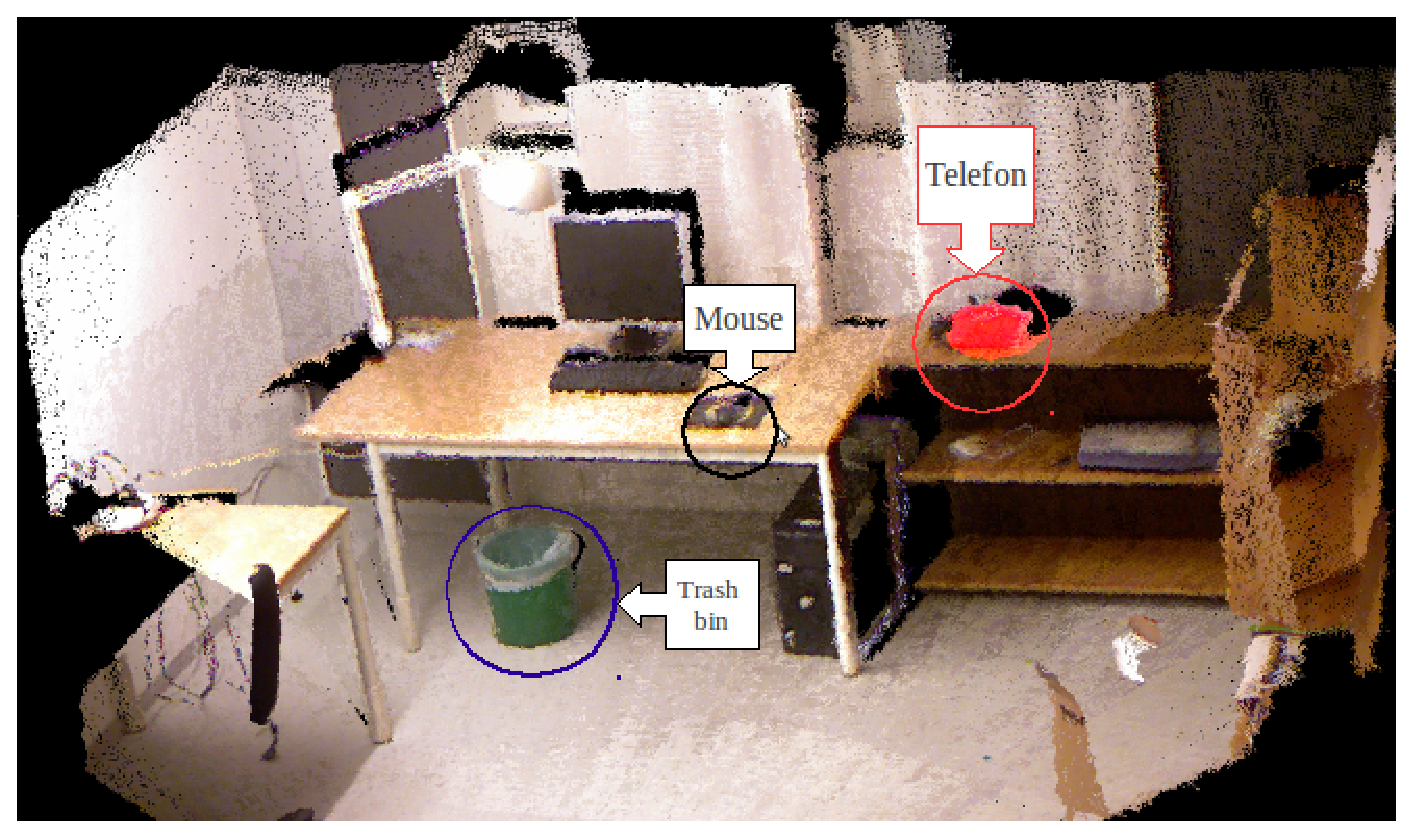
\includegraphics[width=2in,height=2in]{./Figures/518_1_telefon_labels}}
    \subfigure[The same scene with different location of the objects.]{\label{TrainClouds2.figure:tmt2}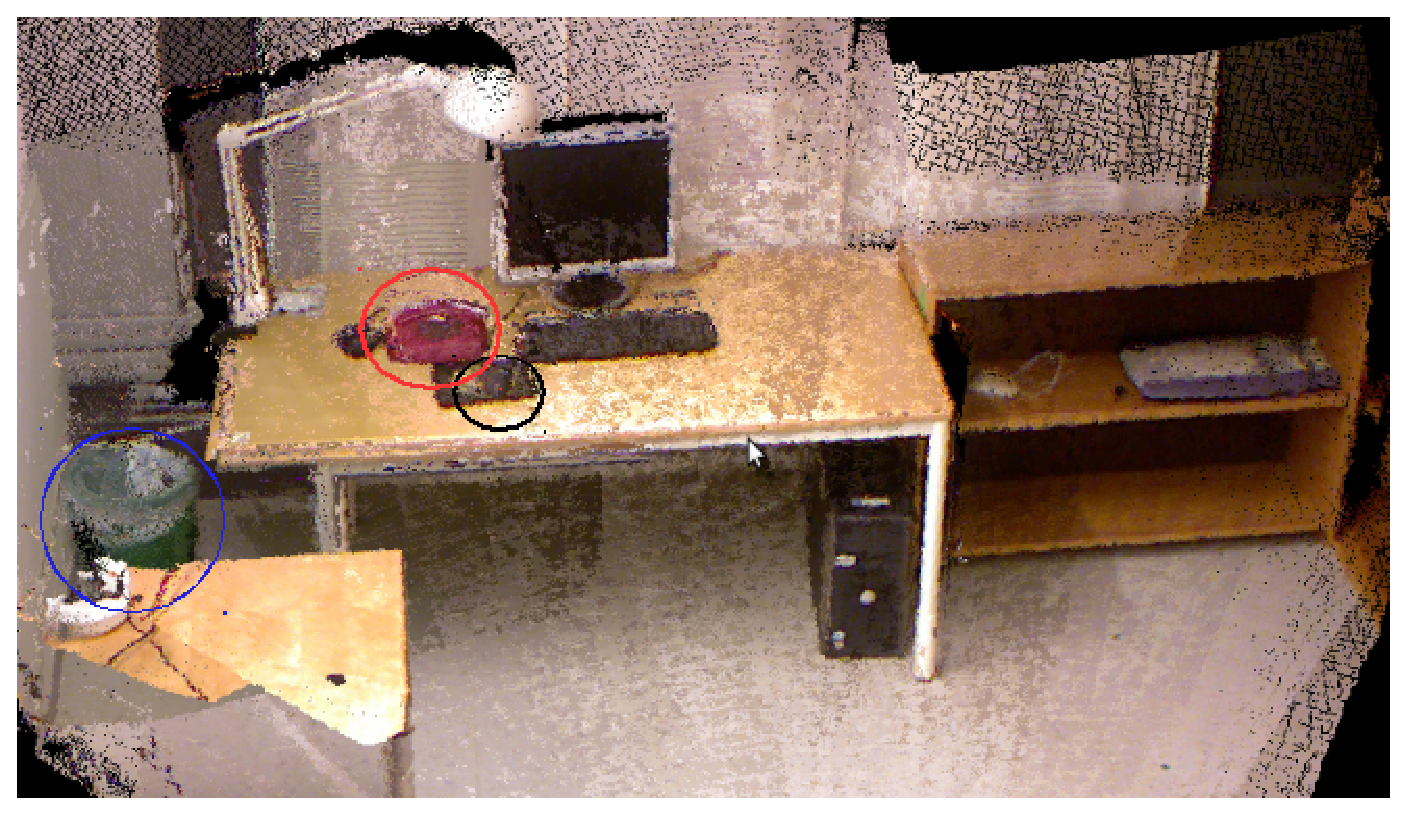
\includegraphics[width=2in,height=2in]{./Figures/518_3_labels}} \\
    \subfigure[Partial cloud including white board wipers.]{\label{TrainClouds2.figure:wiper}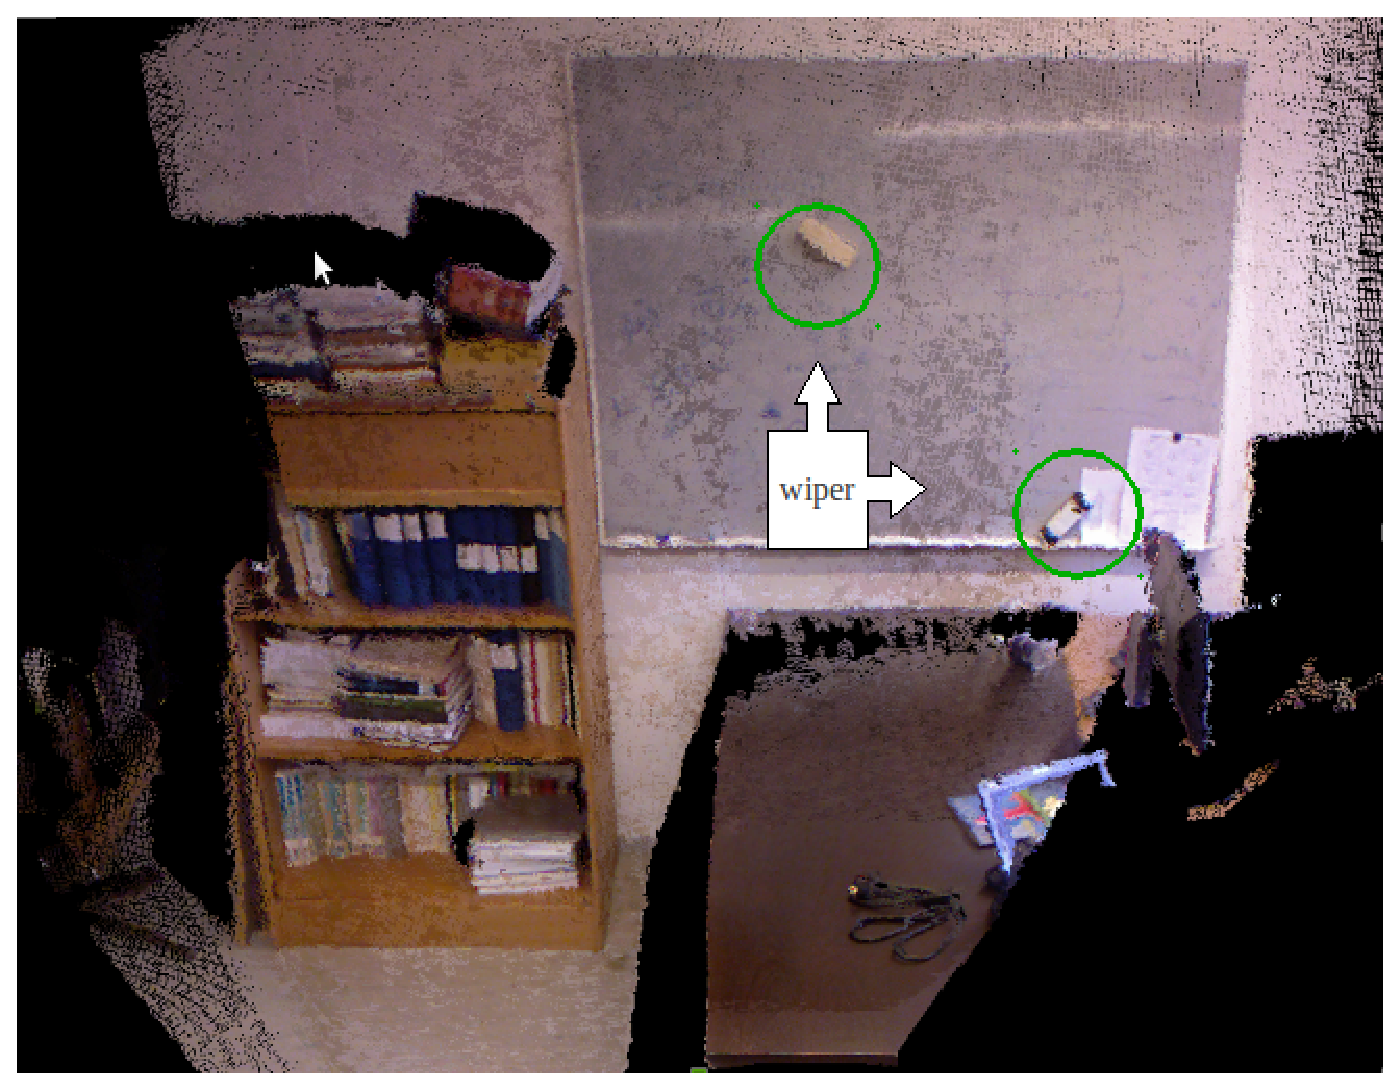
\includegraphics[width=2in,height=2in]{./Figures/wiper_labels}}
    \subfigure[A partial cloud including several instances of 3 object categories.]{\label{TrainClouds2.figure:tmt3}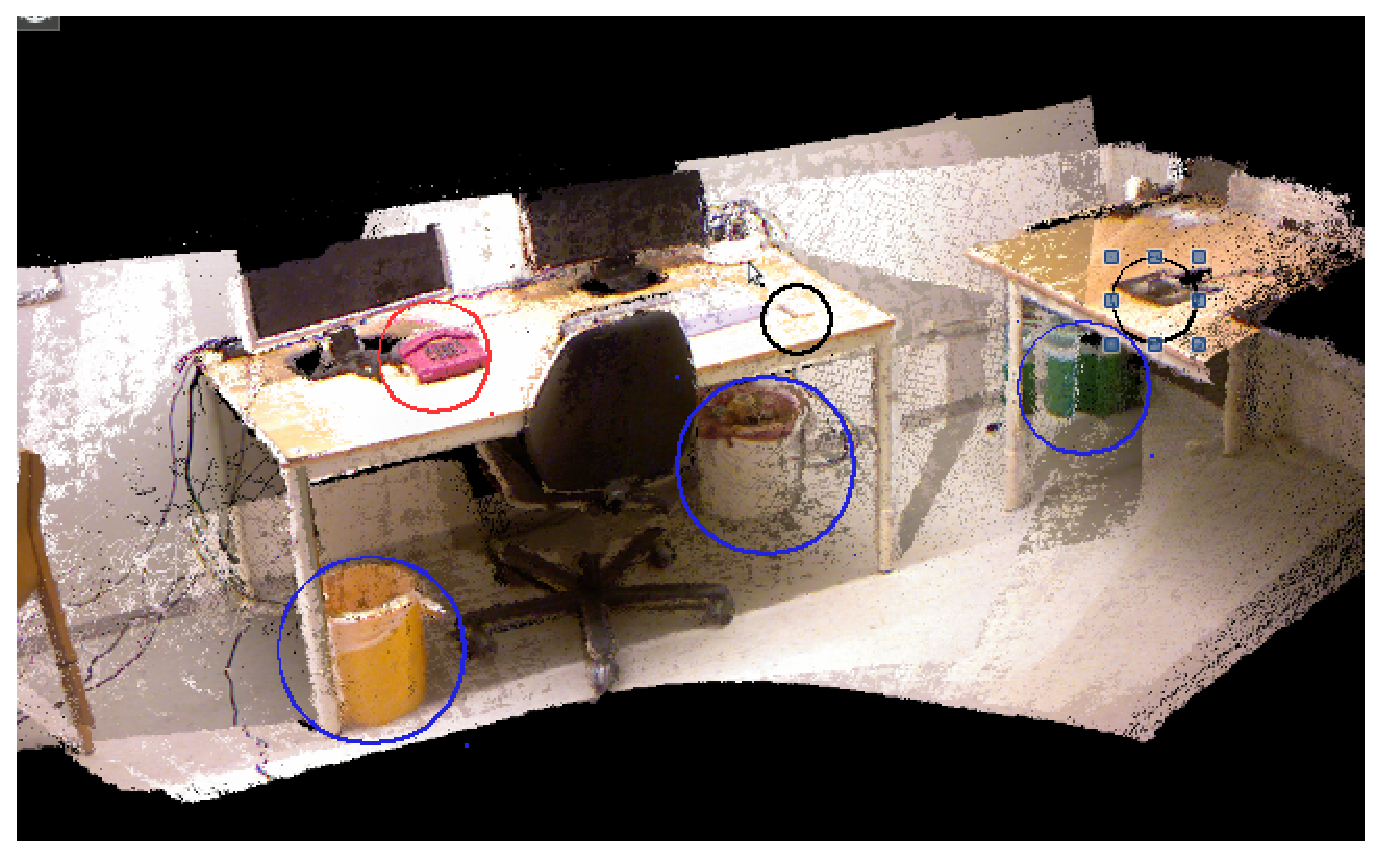
\includegraphics[width=2in,height=2in]{./Figures/518_4_labels}} \\
  \end{center}
  \caption[Train set point-clouds including four different object class.]
  {Partial point-clouds including four object categories: trash bin(marked with blue circles), mouse(back circles), telephone(red circles) and wiper(green circles) in different location settings used in training.(best viewed in color)}
  \label{TrainClouds2.figure:edge}
\end{figure}




After acquiring the point-clouds, some python scripts were used that picks the point-cloud from the input dataset 
and load them into PreProcess module and saves the results of each point-cloud separately in a useful way into the automatically
generated environment. 
Then the annotation tool were used to annotate objects of interest in the point-clouds. 
All point-clouds were annotated with present objects of interest, regardless of them being in the train set or validation to 
make evaluation possible on ones used for test as well. 
Although in validation we would not be using labels from annotation until the end of classification, 
this information is needed for evaluation which would be described later in next Section ~\ref{Results.sec}.


In the next step, another script picks annotated clouds and their normals (estimated in PreProcess) into Feature extract 
and  resulting feature vectors are saved in a folder for the corresponding object class under train or validation set, regarding
which set their source point-cloud belong to.
Then, a subset is randomly selected from the train samples in a way that includes all the positive samples and sevral times more of 
 negative samples to make the train set.
In first experiments for Trash bin we have used train sets with 10 percent positive and 90 percent negative samples.
In later experiments and for other objects train sets are generated with all extracted positive samples and two times more of negative samples.
In these experiments positive sample have a 33\% share in the train set.

At this point, all data sets will be scaled with the same parameters, then the scaled train set is given to SVM train 
to make the models for each of the object class's context. 
During training, different values for the parameters are considered, and each resulting model is applied on samples from validation
set. 
Classification results with different examined values of these parameters are compared and best models are selected. 
The results and evaluation procedure are discussed in Section ~\ref{Results.sec}.

\section{Results}
\label{Results.sec}
% Definitions and metrics
In this Section, we take a look at some results and Analise and evaluate them to see how good our method performs.
It can help if we first check some plots showing how does the feature vector look like and how discriminative it can be.
Figures ~\ref{CompareNegHis.figure} and ~\ref{ComparePosHist.figure} show the plot of two random negative and two random 
positive samples.   
% Results
\begin{figure}[t]
  \centerpsw{CompareNegHis}{0.65\columnwidth}
  \caption[Compare two random negative samples]
  {Two random Negative samples plotted on top of each other to compare.}
  \label{CompareNegHis.figure}
\end{figure}

\begin{figure}[t]
  \centerpsw{ComparePosHist}{0.65\columnwidth}
  \caption[Compare two random Positive samples]
  {Two random Positive samples plotted on top of each other to compare.}
  \label{ComparePosHist.figure}
\end{figure}


In order to have a more clear idea about differences between samples, we can also look at the distances between random samples
in the same class and compare them to the distance of samples from different classes. 
Figure ~\ref{DistanceOFTwoNegHist.figure} shows the distance in two random negative samples. 
It should be noticed that the first part of the plot reflects the view point component of the feature vector.
 
\begin{figure}[t]
  \centerpsw{DistanceOFTwoNegHist}{0.65\columnwidth}
  \caption[Distance between random negative samples]
  {Distance between random negative samples.}
  \label{DistanceOFTwoNegHist.figure}
\end{figure}

And figure ~\ref{DistanceOFTwoPosHist.figure} is the same plot for positive samples. 
Features extracted for each class can have big differences as well, which was predictable. 
Considering different surfaces captured as context by these features that can belong to a class causes the differences. 
A positive sample can be representing, for instance, the surface of a table or a wall or the meeting region of these two surfaces. 
This comparison gives us an idea about how challenging it is to train a classifier for such data.
As mentioned before, it is also important that more attention to be put on learning the positive samples rather than negative ones. 

\begin{figure}[t]
  \centerpsw{DistanceOFTwoPosHist}{0.65\columnwidth}
  \caption[Distance between random Positive samples]
  {Distance between random Positive samples.}
  \label{DistanceOFTwoPosHist.figure}
\end{figure}

Figure ~\ref{DistanceOFPosandNegHist.figure} is showing the distance between random positive and negative samples.

\begin{figure}[t]
  \centerpsw{DistanceOFPosandNegHist}{0.65\columnwidth}
  \caption[Distance of Positive and Negative samples]
  {Distance between random positive and negative samples.}
  \label{DistanceOFPosandNegHist.figure}
\end{figure}


\subsection{Evaluation}
\label{Evaluation.ssec}

%As mentioned before there could be negative samples in train set that are labeled as negative just because they were not captured 
%from a neighborhood of an annotated object while they have very similar features to positive samples. 
%Such samples need to be predicted as positive. 

Here we define a metric and an evaluation method that we considered in this work.
Metrics such as accuracy of prediction is not something that can show the performance of our system.
Accuracy is measuring number of samples that are correctly classified with respect to the total number of samples.
Here we do not have direct access to the number of correct classification. 

Based on the problem definition, we are looking for possible context of an object, which regards to locations that an object 
is expected to be found, not just location that an object is present.
Intuitively, set of points that belong to an actual object (if there is an actual object in the scene) is a subset of all possible 
object points in that scene.
Therefore, actual object points ($Lp$) are a subset of predicted positive points ($Pp$) if the model and classifier perform well 
(equation \ref{Lp-PpRelation.eq}).

\begin{equation}
 \label{Lp-PpRelation.eq}
 Lp \subset Pp
\end{equation}

In other words, from a good result, we expect any random point sampling which is an actual object point to be within predicted 
positive points.   
%if the predictions give us points of the point-cloud where there is a high probability of finding the object, it
%would be what we want. 
%The point here is, that the location of the object would be a subset of this predicted set. 
With this definition there would be a problem: if all points get predicted as positive then actual object points would definitely 
be a subset of it, while our classification has failed.
As a result, we define a good result as predicted set of locations that reduces our search space for the object as much as possible 
while it preserves the high probability of finding the object.

Equation ~\ref{Eval.eq} shows the evaluation metric, where $E(\tau)$ is the the value of the metric with respect to a probability 
threshold $\tau$. 
This threshold sets the boundary for the lowest probability value that the prediction should have, so that the sample can be 
considered as positive. 
This threshold is assigned with a value in a loop that as a result in each iteration a top fraction of the samples are being picked
and analyzed. 
For instance we will pick top five percent of the samples and measure how much would be the probability of having the object in 
this fraction.

The threshold is computed based on an increasing value of the number of samples that are considered.
$Pp_{\tau}$ is Predicted positive sample with respect to the value if the threshold and $n(x)$ is the number of $x$. $Lp$ is the 
Labeled positive in the data-set or in other word the annotated object.

\begin{equation}
 \label{Eval.eq}
    E(\tau) = \frac{n({Pp_{\tau}} \cap {Lp})}{n(Lp)} 
\end{equation}

This value is between zero and one, and a value closer to one, while the threshold is high enough, shows a better result.
This metric is also used in experiments to find the best models and parameters. 
Here we also translate the sample base results into point base which means the result is assigned to the point for which the sample
is taken.
Therefore, the prediction directly shows if a candidate OPoint is a possible object point or not.

Figure ~\ref{Eval80ExperimentTop10.figure} shows the value of $E$ for top ten percent of the points with respect to their 
prediction probability in experiments with 80 different configuration of weights and gamma.
As it can be seen the results look pretty good.

\begin{figure}[t]
  \centerpsw{Eval80ExperimentTop10}{0.65\columnwidth}
  \caption[Evaluation result of 80 experiments]
  {Top 10 percent of positive predictions in experiments with 80 different configurations for parameters.}
  \label{Eval80ExperimentTop10.figure}
\end{figure}

Considering best models, it can be inferred from the curves that for instance, top five percent of the points contains twenty 
percent of the object which is a very good result. 
In other words, reducing the the search space to only 5 percent we still have four time chance of finding the object.

Figure ~\ref{evalSevenExp.figure} shows this evaluation for seven experiments with different weights for class -1. 
The value is depicted with respect to the fraction of points considered.

\begin{figure}[t]
  \centerpsw{evalMorevalues}{0.65\columnwidth}
  \caption[Evaluation diagram(1)]
  {Evaluation diagram(1)}
  \label{evalSevenExp.figure}
\end{figure}

Figure ~\ref{TrashPrediction.figure:edge} shows the prediction of trash bin context on a full pointcloud of an office. 
The marked region shows the points with highest probability values.

\begin{figure} [htp]
   \begin{center}
    \subfigure[A test point-cloud for trash bin model, marked region with red circle is the predicted context.]{\label{TrashPrediction.figure:full}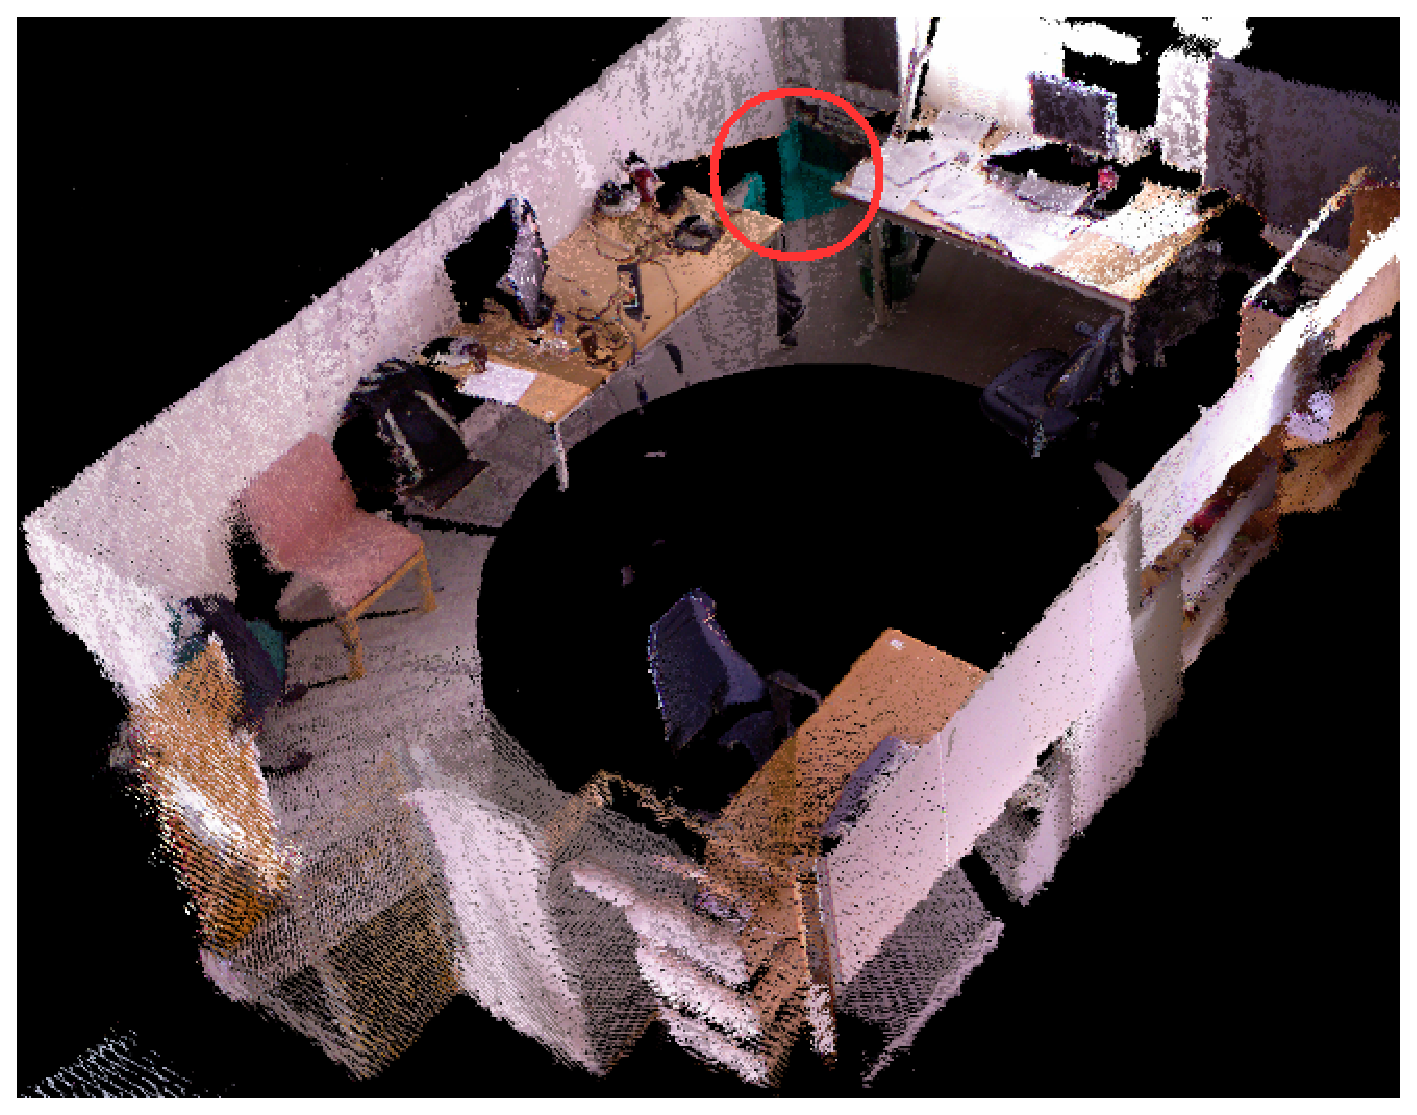
\includegraphics[width=3in,height=3in]{./Figures/TrashBinPrediction}}
    \subfigure[Focused to predicted region.]{\label{TrashPrediction.figure:focused}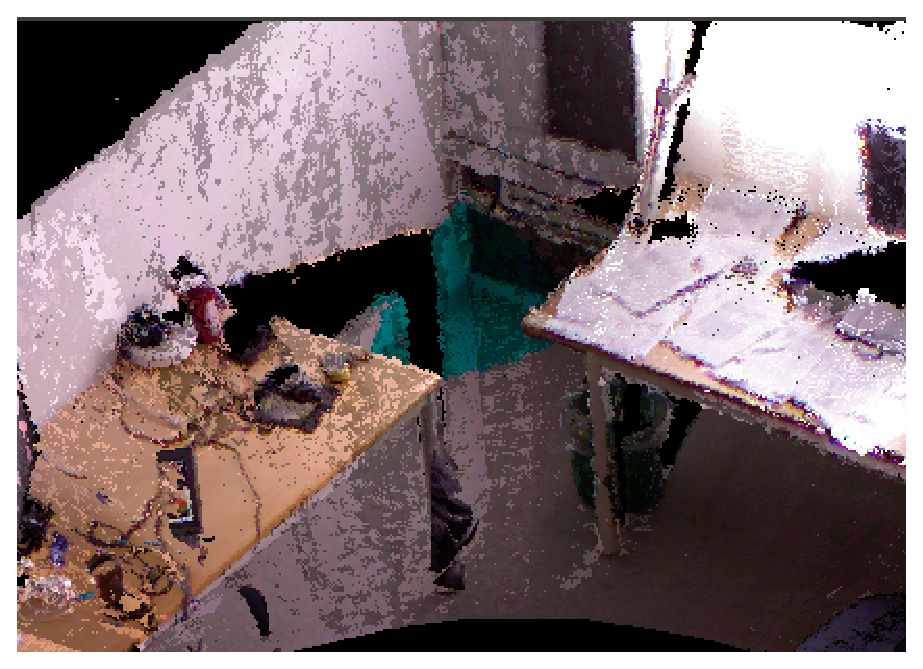
\includegraphics[width=3in,height=3in]{./Figures/TrashBinPrediction_focused}} \\
  \end{center}
  \caption[Prediction of Trash bin model.]
  {Prediction of Trash bin context on a full point-cloud of an office. The marked region shows the points with highest probability values.(best viewed in color)}
  \label{TrashPrediction.figure:edge}
\end{figure}

\begin{figure} [htp]
   \begin{center}
    \subfigure[Predicted context for Mouse.]{\label{ContextPrediction_518_1.figure:wiper}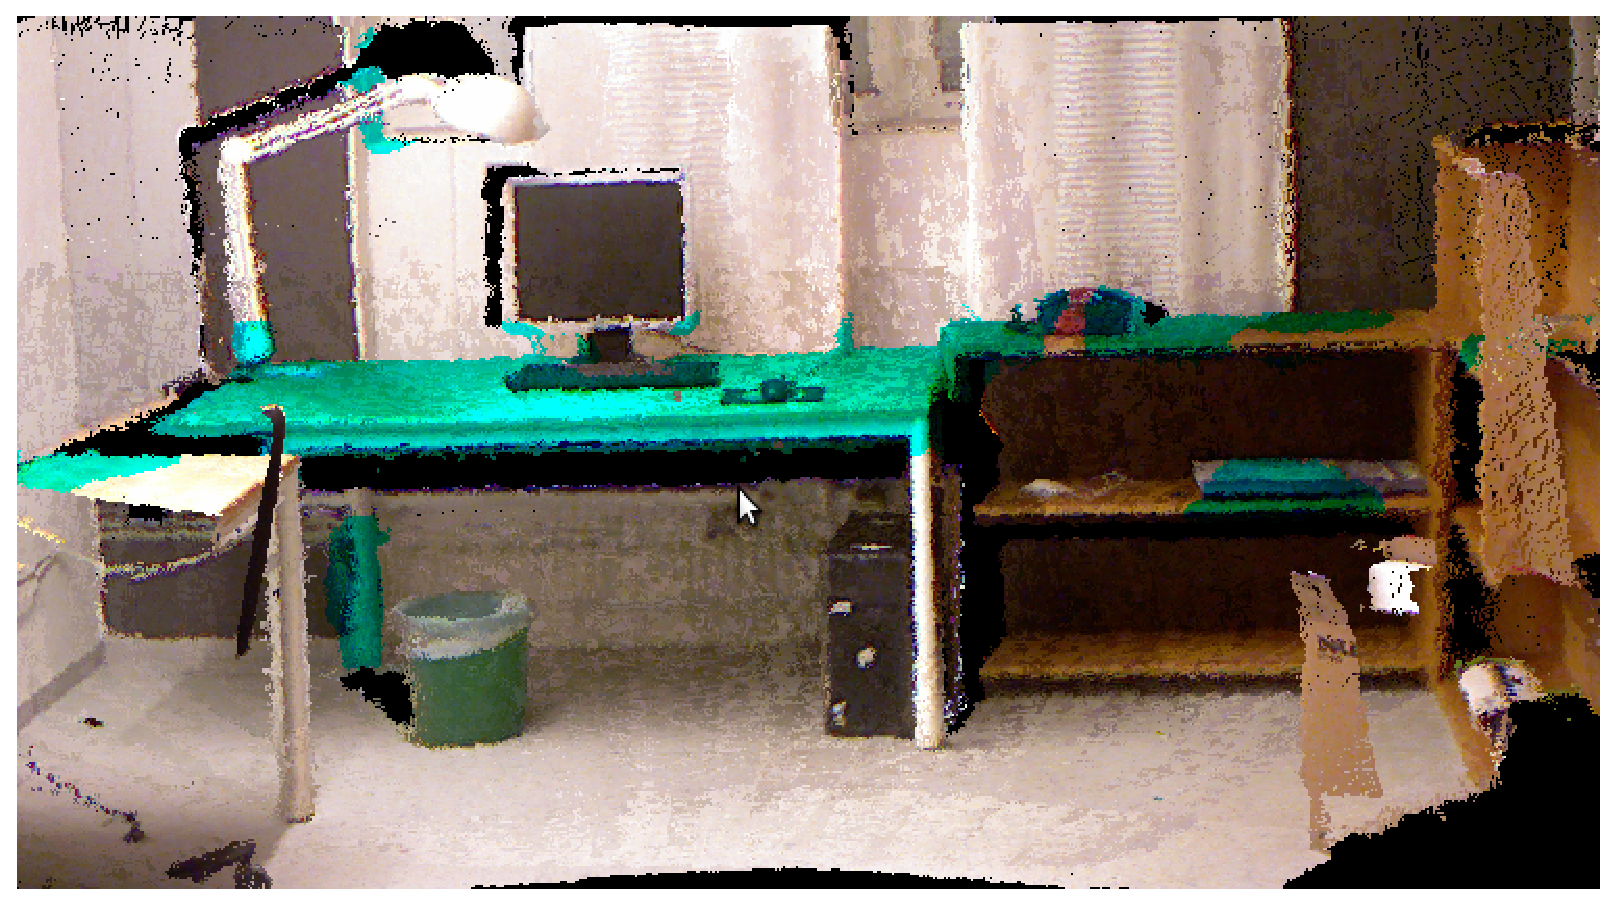
\includegraphics[width=2in,height=2in]{./Figures/518_1_MousePrediction_c1g0}}
    \subfigure[Predicted context for white-board wiper.]{\label{ContextPrediction_518_1.figure:mouse}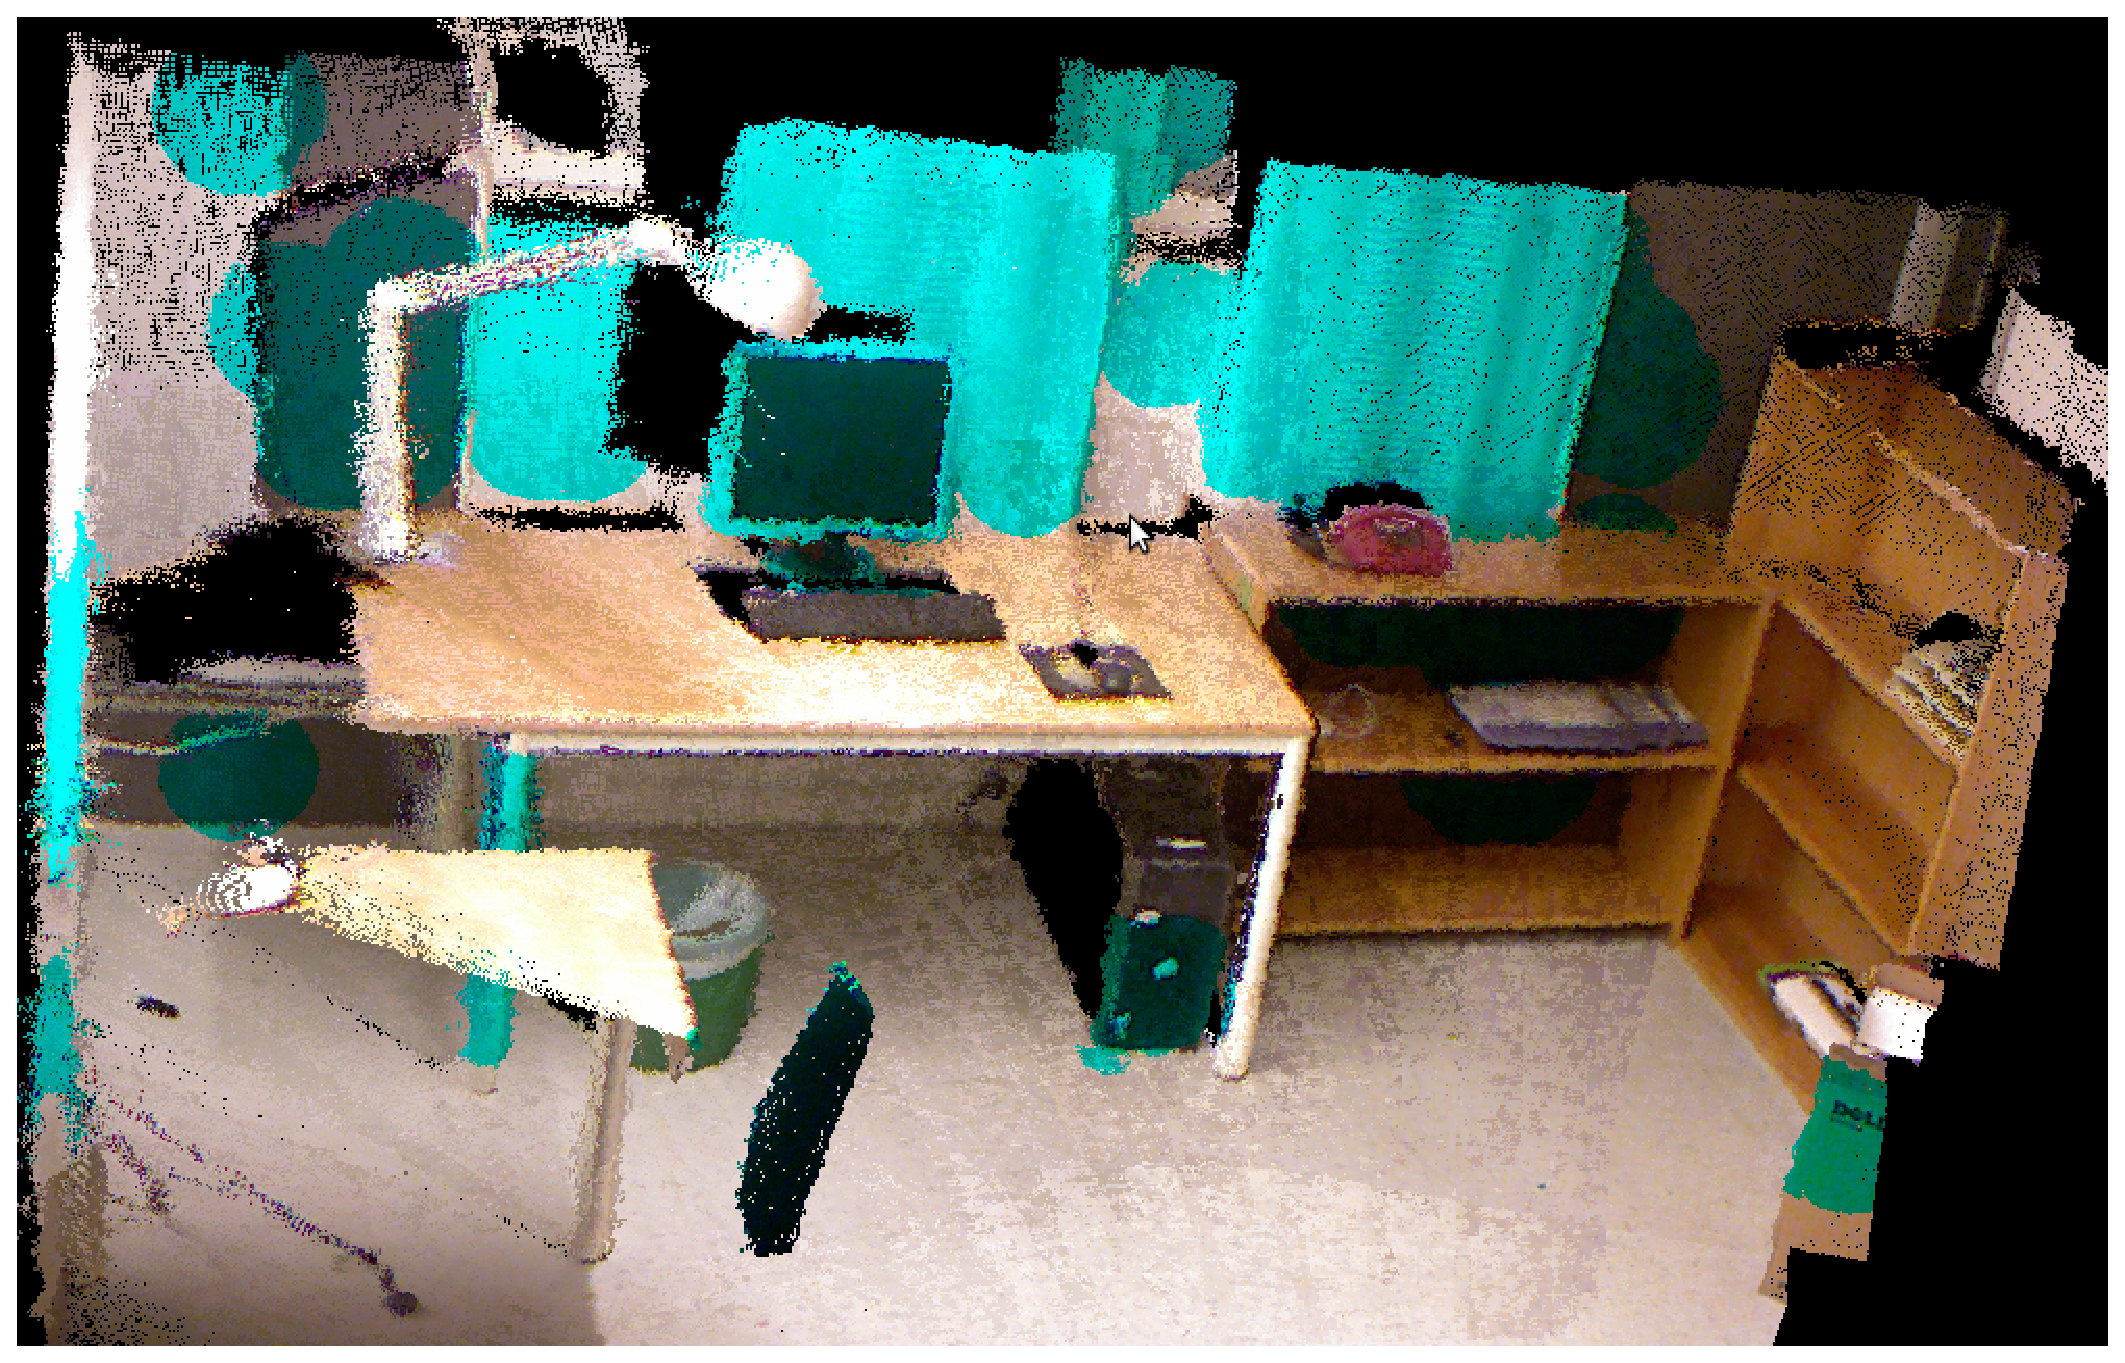
\includegraphics[width=2in,height=2in]{./Figures/518_1_WiperPrediction_c1g0}} \\
    \subfigure[Predicted context for Telephone.]{\label{ContextPrediction_518_1.figure:Telephone}\includegraphics[width=2in,height=2in]{./Figures/518_1_TelefonPrediction_c1g0}}
    \subfigure[Predicted context for Trash Bin.]{\label{ContextPrediction_518_1.figure:TrashBin}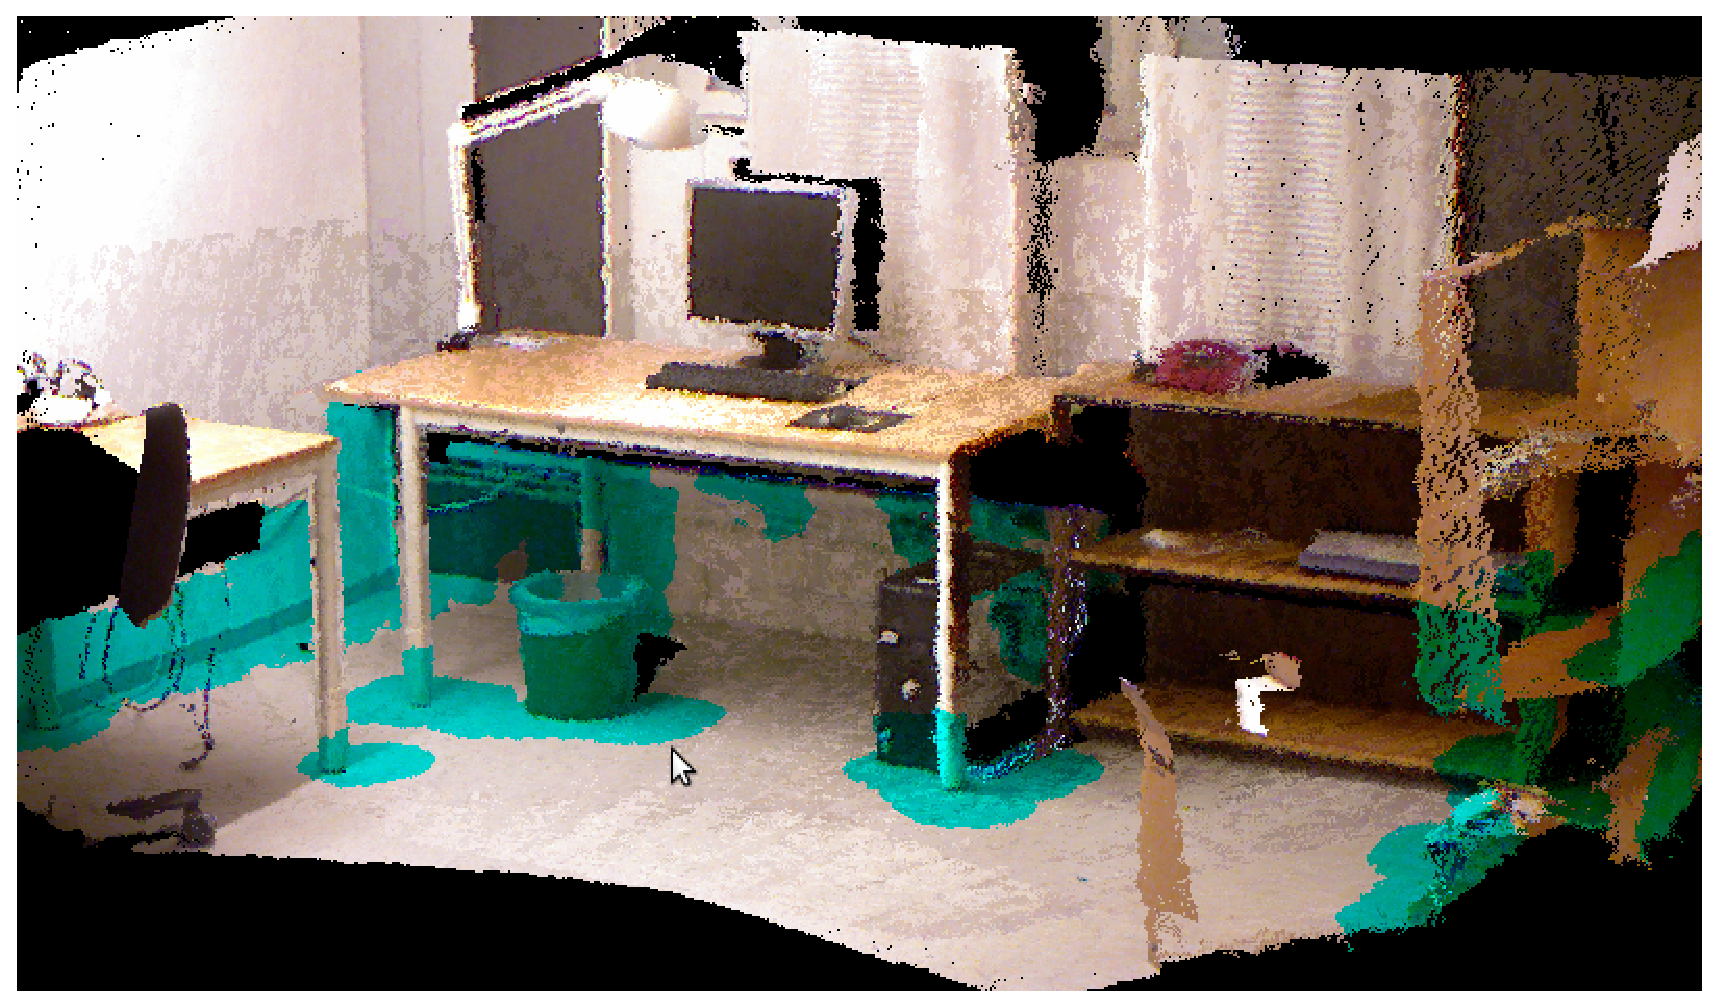
\includegraphics[width=2in,height=2in]{./Figures/518_1_TrashBinPrediction_c1g0}} \\
  \end{center}
  \caption[Visualization of context model prediction on sample cloud 1.]
  {Visualization of context model prediction on sample cloud 1 for four objects. The key point predicted as positive and the blob around it is projected on the point-cloud in cyan color.(best viewed in color)}
  \label{ContextPrediction_518_1.figure:edge}
\end{figure}

In figure ~\ref{ContextPrediction_518_1.figure:edge}, the predicted contexts of four object used in experiments 
are projected on the point-cloud of an office. 
It should be noticed that the regions shown in cyan, are blobs with a key point in the center which is predicted as 
context.


% 
% \begin{figure}[t]
%   \centerpsw{Eval80Experiment}{0.65\columnwidth}
%   \caption[]
%   {}
%   \label{}
% \end{figure}
% 
% 
% \begin{figure}[t]
%   \centerpsw{log(w1w-1)}{0.65\columnwidth}
%   \caption[]
%   {}
%   \label{}
% \end{figure}
% 
% \begin{figure}[t]
%   \centerpsw{PositiveRatio}{0.65\columnwidth}
%   \caption[]
%   {}
%   \label{}
% \end{figure}
% 
% \begin{figure}[t]
%   \centerpsw{TruePositiveRatio}{0.65\columnwidth}
%   \caption[]
%   {}
%   \label{}
% \end{figure}
% 
% \begin{figure}[t]
%   \centerpsw{w1w-1}{0.65\columnwidth}
%   \caption[]
%   {}
%   \label{}
% \end{figure}
% 
% 
